\chapter{Theoretical motivation}

\begin{chapquote}{Thomas Khun, \emph{The Structure of Scientific Revolutions}}{Surveying the rich experimental literature from which these examples are drawn makes one suspect that something like a paradigm is prerequisite to perception itself.}
\end{chapquote}

\section{The Standard Model}

SU(3) x SU(2) x U(1) gauge interactions

\begin{figure}
\centering
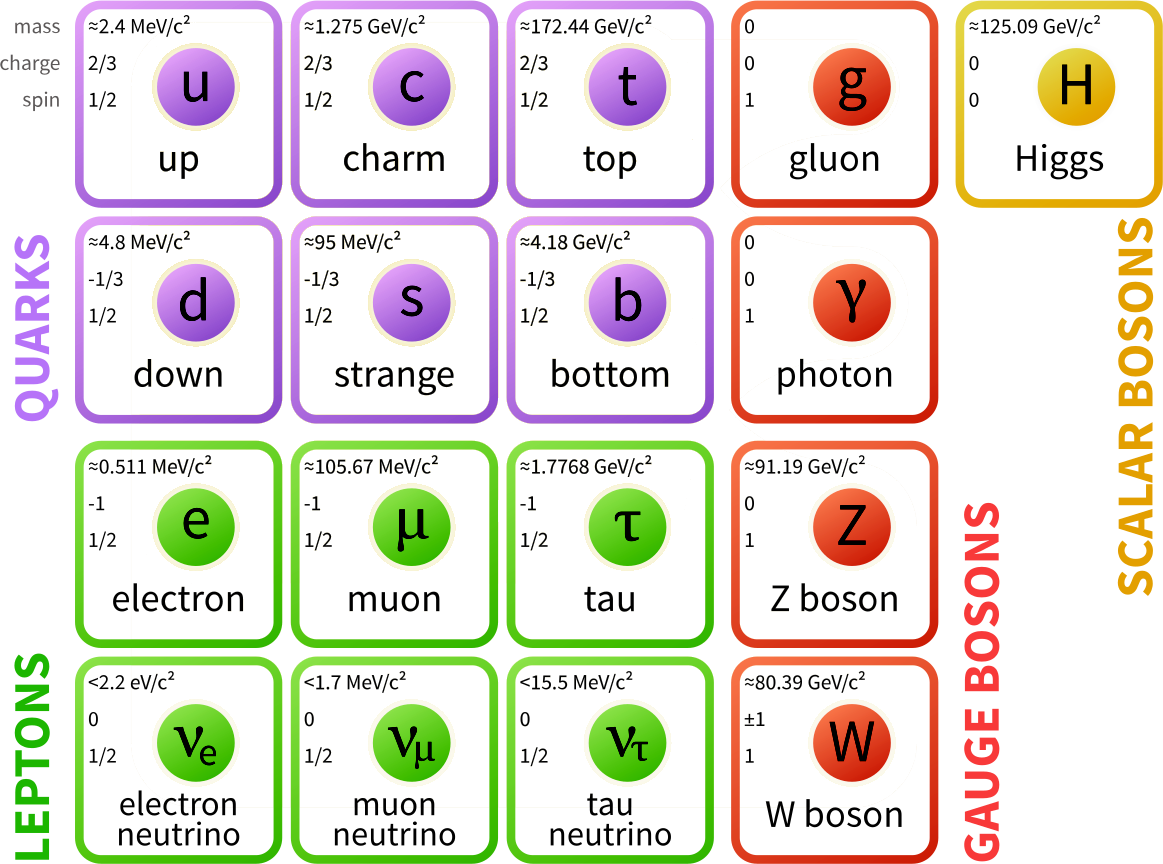
\includegraphics[width=.7\textwidth]{figures/intro/SM-Particles.png}
\caption{\cite{wiki-sm}}
\label{fig:SM-Particles}
\end{figure}

\begin{equation}
\mathcal{L}_{SM} =  - \frac{1}{4} F_{\mu \nu} F^{\mu \nu} + i \bar{\psi} \gamma_\mu D^\mu \psi + \left( y_{ij} \bar{\psi}_i \psi_j + h.c. \right) + |D^\mu \phi|^2 - V (\phi)
\label{eq:sm}
\end{equation}

%I think the

\begin{figure}
\centering
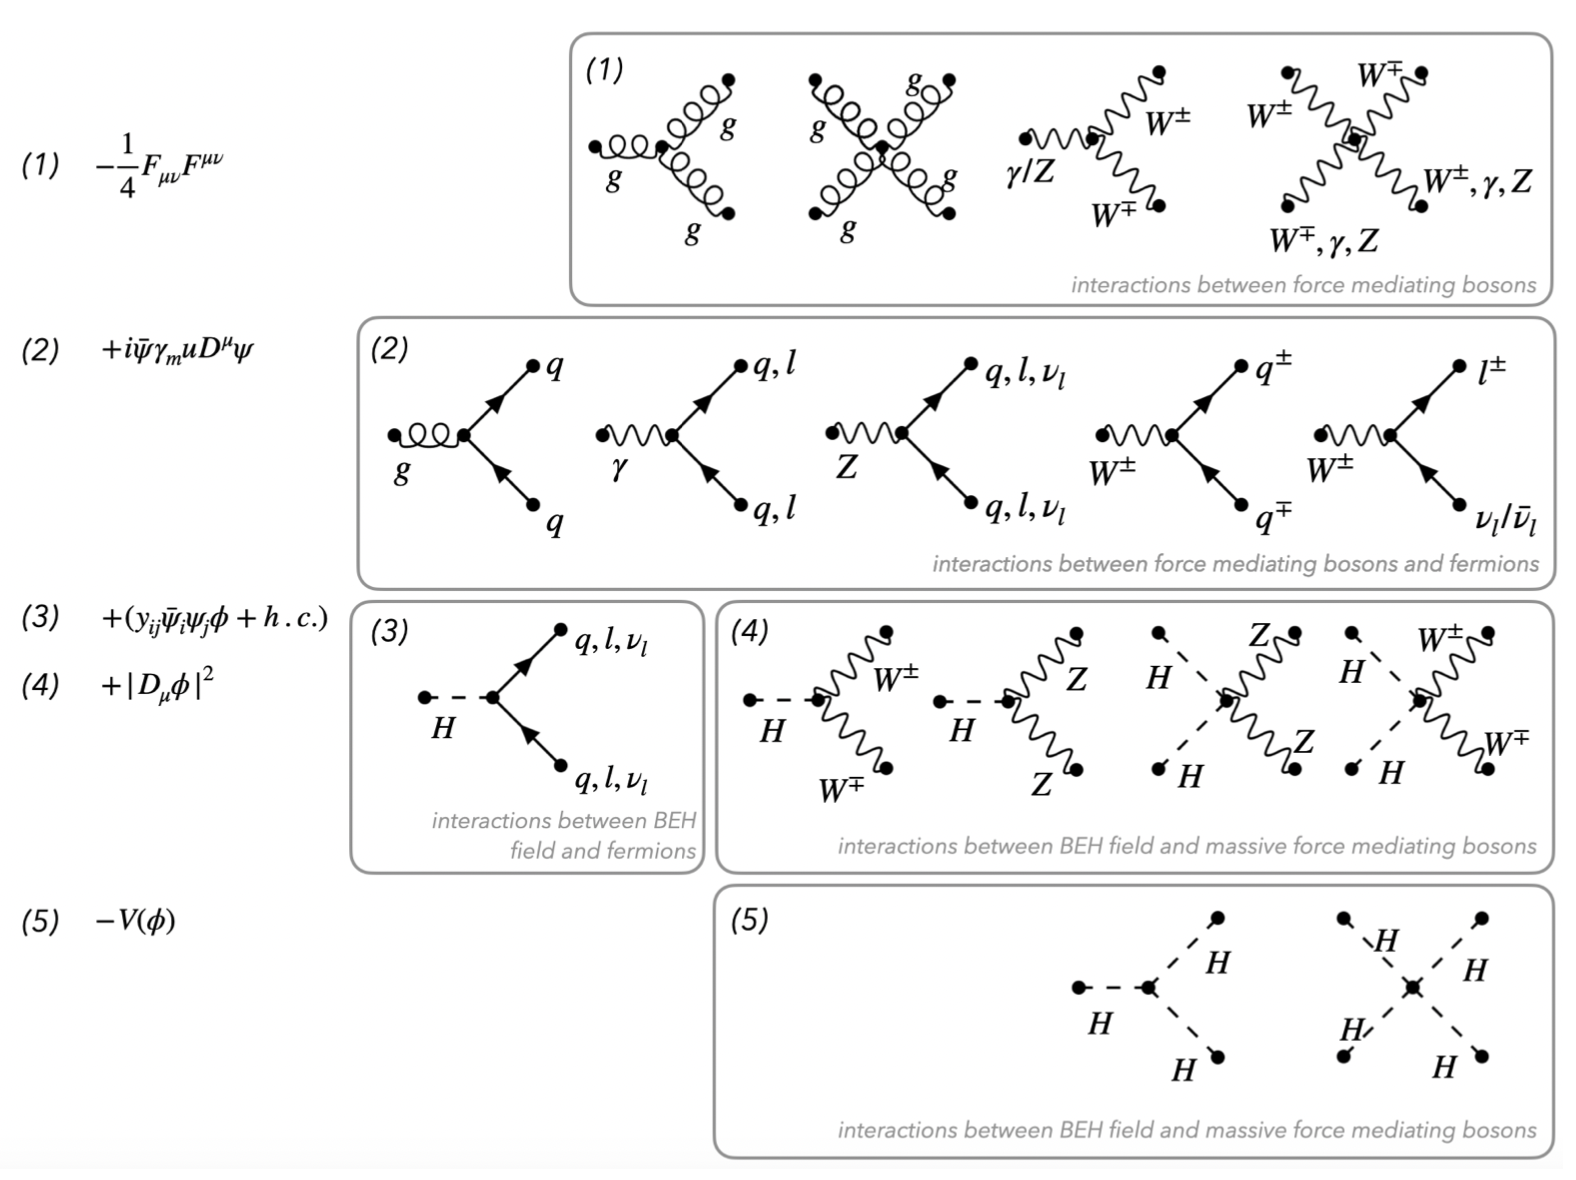
\includegraphics[width=\textwidth]{figures/intro/mel-sm-diagrams.png}
\caption{\cite{Melissa-thesis}}
\label{fig:mel-sm}
\end{figure}

\section{The Higgs mechanism}
I heard from Dale that the pdg is a v good ref for this!!

\section{Effective Field Theories to search for new physics}

\section{Status of the experimental HH results}

\begin{figure}
\centering
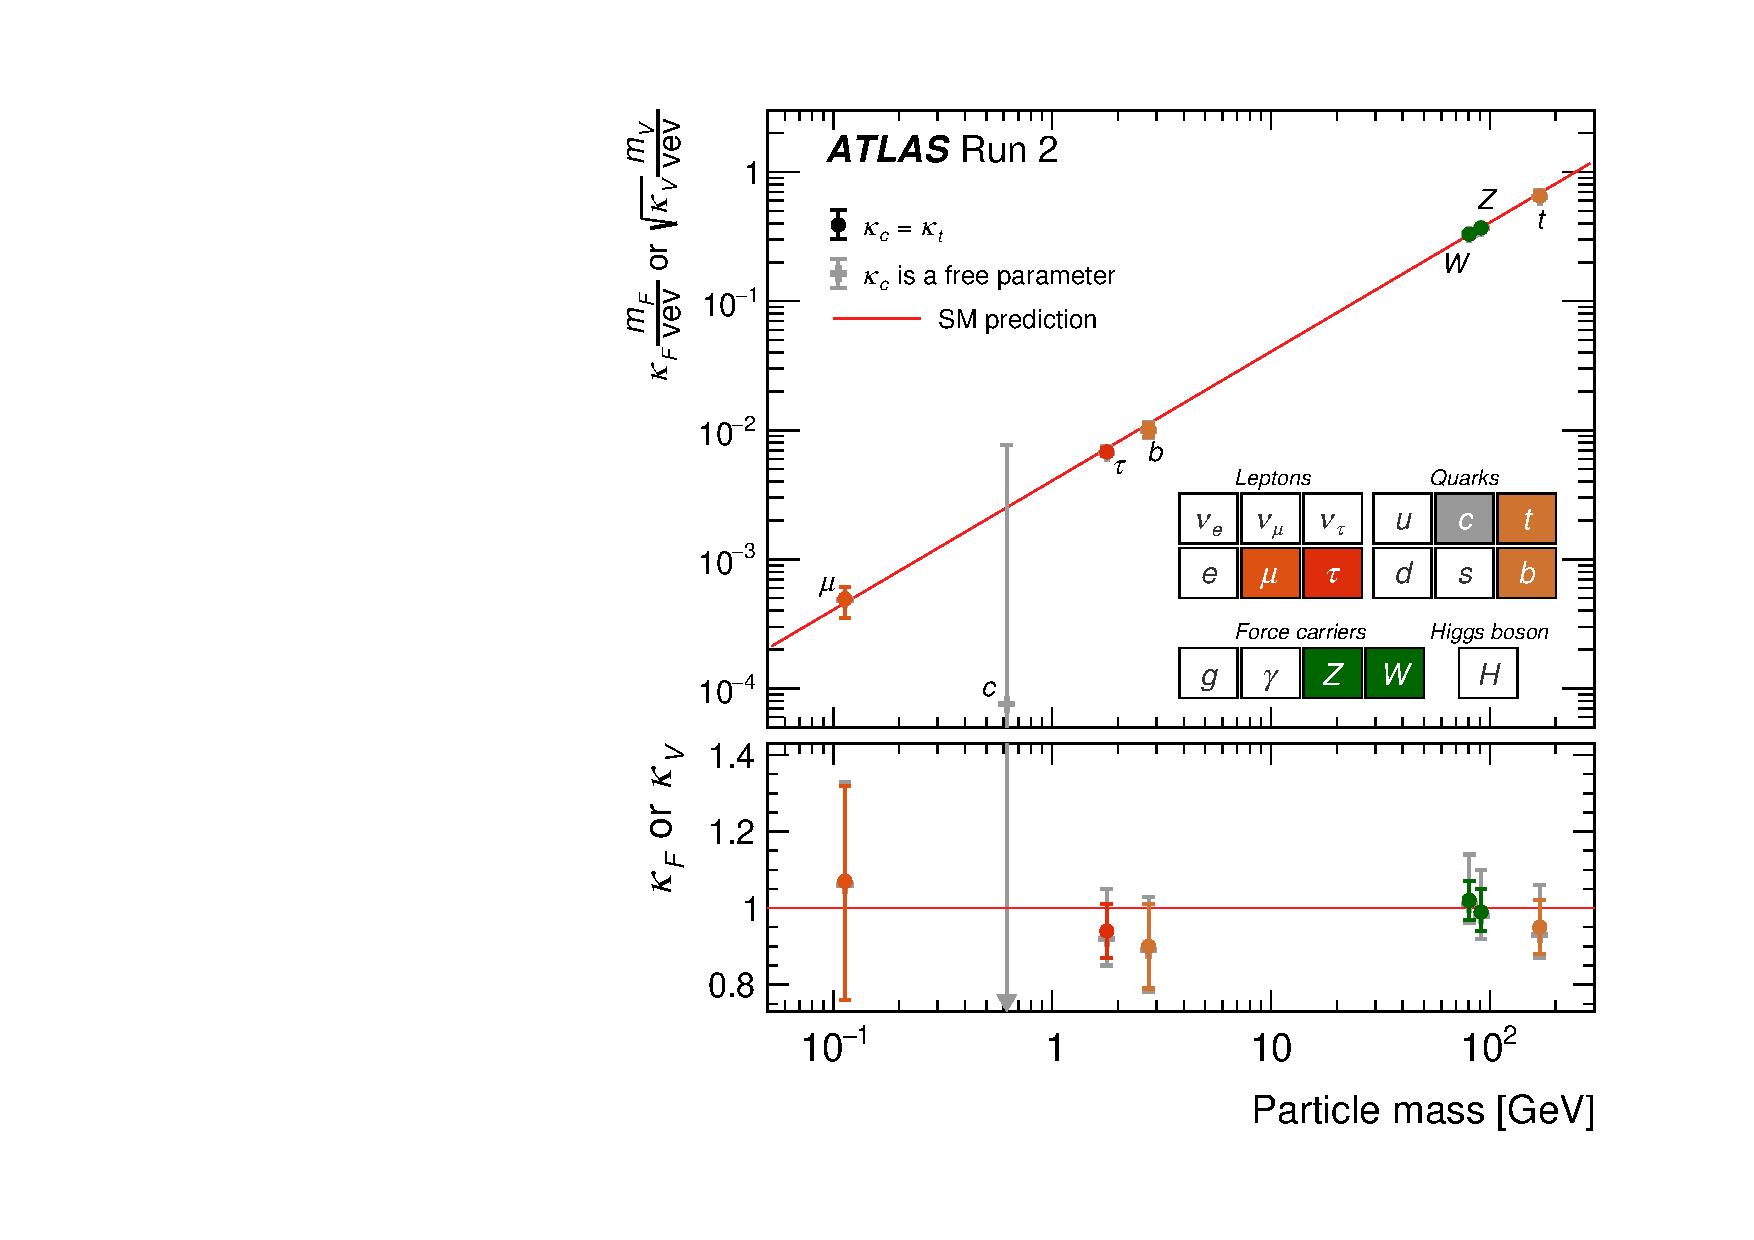
\includegraphics[width=.7\textwidth]{figures/intro/atlas-nature-10yrs/fig_05}
\caption{\cite{2207.00092}}
\label{fig:pcle-mass-atlas}
\end{figure}
